\documentclass{bakalarka}
\usepackage[utf8]{inputenc} 
\usepackage[czech]{babel}
\usepackage{ae}
\usepackage{fancyhdr}
\usepackage{graphicx}
\usepackage{float}
\usepackage{eurosym}
\usepackage{longtable}
\usepackage{subcaption}
\usepackage{enumitem}
\usepackage{listings}
\usepackage{color}
\usepackage[colorlinks=true]{hyperref}

\definecolor{brown}{rgb}{.33,.28,0}
\definecolor{gray}{rgb}{.3,.42,.45}
\definecolor{darkRed}{rgb}{.51,0,.12}
\definecolor{tyrk}{rgb}{.4,.8,.75}
\definecolor{darkGreen}{rgb}{0,.51,.12}

\renewcommand{\lstlistingname}{Kód}

\lstnewenvironment{lstpython}[2][]{\lstset{
	#1,
	#2,
	language=Python,
	frame=single,
	showstringspaces=false,
	stringstyle=\color{darkRed},
	commentstyle=\color{gray},
	numberstyle=\color{brown},
	keywordstyle=\color{tyrk},
	morekeywords={open, focus, wait, paste, type, click, find, popup, popError, exists, close, right, text, targetOffset},
	keywordstyle=[2]\color{red},
	keywords=[2]{App, Key},
	keywordstyle=[3]\color{brown},
	keywords=[3]{ENTER}
}}{}
\lstnewenvironment{lstjava}[2][]{\lstset{
	#1,
	#2,
	language=Java,
	frame=single,
	showstringspaces=false,
	commentstyle=\color{darkGreen},
	keywordstyle=\color{blue},
	stringstyle=\color{red}
}}{}



\usepackage{verbatim}

\author{Jaroslav Klaus}
\title{Využití nástrojů pro testování grafického uživatelského rozhraní}
\titlet{}
\titlett{}
\university{Západočeská univerzita v~Plzni}
\faculty{Fakulta aplikovaných věd}
\department{Katedra informatiky a~výpočetní techniky}
\subject{Projekt 5}
\town{Plzeň}
\begin{document}
\pagestyle{fancy}
\renewcommand{\chaptermark}[1]{\markboth{\textit{#1}}{}}
\renewcommand{\sectionmark}[1]{\markright{\textit{#1}}{}}
\cfoot{\thepage}
\lhead{\leftmark}
\rhead{\rightmark}
\maketitle
\begin{comment}
\chapter*{Prohlášení}
\thispagestyle{empty}
Prohlašuji, že jsem práci vypracoval samostatně a~výhradně s~použitím citovaných pramenů.
\vskip 1.5em
V~Plzni dne \today
\vskip 0.7em
\hskip 9cm Jaroslav Klaus
\chapter*{Abstract}
\thispagestyle{empty}
This paper deals with the use of software tools for testing graphical user interface. It compares some of the tools and describes the use of one of them in a~way that fits into the subject KIV/OKS.
\chapter*{Abstrakt}
\thispagestyle{empty}
Tato práce se zabývá využitím nástrojů k~testování grafického uživatelského rozhraní aplikací. Srovnává některé nástroje k~tomu určené a~popisuje použití jednoho z~nich tak, aby svou filosofií zapadal do předmětu KIV/OKS.
\end{comment}
\tableofcontents
\pagestyle{fancy}
\renewcommand{\chaptermark}[1]{\markboth{\textit{#1}}{}}
\renewcommand{\sectionmark}[1]{\markright{\textit{#1}}{}}
\cfoot{\thepage}
\lhead{\leftmark}
\rhead{\rightmark}
\parskip 1em
\chapter{Úvod}
Testování aplikací je nedílnou součástí jejich vývoje a~v~dnešní době se tomuto oddílu tvorby aplikací věnuje čím dál více pozornosti. Dá se rozdělit do různých skupin, např. podle toho, kdy se testování provádí, jakým způsobem se provádí, jak se k~testované aplikaci přistupuje, či jaká část aplikace se podrobuje testům.

Jednou z~důležitých součástí je testování grafického uživatelského rozhraní. Zde se testeři soustředí na to, zda daná aplikace vypadá tak, jak to požadují vývojáři a~návrh, a~zda grafické prvky správně fungují. Dále se zaměřuje na to, zda je aplikace přívětivá k~uživateli a~práce s~ní není příliš komplikovaná.

Při testování grafického uživatelského rozhraní se může spousta testů mnohokrát opakovat, a~proto je snaha tyto testy nějak automatizovat. K~tomu se může využít některý z~nástrojů k~tomu určený. Cílem této práce je seznámit se s~některými z~těchto nástrojů, jeden z~nich vybrat a~pomocí něj vytvořit sadu ukázkových testů svou filosofií zapadajících do předmětu KIV/OKS.

\chapter{Přehled nástrojů}
V~této kapitole následuje přehled nástrojů a~některých jejich vlastností. V~tabulce \ref{PrehledNastroju} je uveden název nástroje, jeho licence resp. cena, jazyk, ve kterém se testy píší, platforma, na které nástroj funguje a~která GUI je nástroj schopen testovat. Z~bezplatných multiplatformních nástrojů jsem si vybral tři a~ty podrobněji prozkoumal a~porovnal, viz následující kapitola.
{\scriptsize
\begin{longtable}{|l|l|l|l|l|l|}
	\captionsetup{font=normalsize}
	\caption{Přehled nástrojů}
	\label{PrehledNastroju}
		\\\hline
		\textbf{Název}&\textbf{Licence/Cena}&\textbf{Skriptovací jazyk}&\textbf{Platforma}&\textbf{\shortstack{\\Jazykové\\omezení}}\\\hline\hline
		AutoIt\cite{AutoIt}&Freeware&BASIC-like&Windows&-\\\hline
		AutoHotKey\cite{AutoHotKey}&GNU GPLv2&AutoHotKey&Windows&-\\\hline
		AutoKey\cite{AutoKey}&GNU GPLv3&Python&Linux&-\\\hline
		\shortstack{\\SikuliX\cite{Sikuli}\\\cite{SikuliX}}&MIT License&Python, Ruby&\shortstack{\\Windows,\\Linux, Mac}&-\\\hline
		Jubula\cite{Jubula}&EPL 1.0&\shortstack{\\Drag \& Drop,\\Java}&\shortstack{\\Windows,\\Linux, Mac}&\shortstack{\\Java, HTML,\\.NET, iOS} \\\hline
		\shortstack{Robot\\Framework}\cite{RobotFramework}&\shortstack{Apache\\License 2.0}&Natural-like&\shortstack{\\Windows,\\Linux, Mac}&\shortstack{\\Podle pluginů\\(Java, web,\\Android, iOS,\\\dots)}\\\hline
		Squish\cite{Squish}&\shortstack{\\cca\\\EUR{2400}/osoba}&\shortstack{\\Python, JavaScript,\\Ruby, Perl, Tcl}&\shortstack{\\Windows,\\Linux, Mac}&-\\\hline
		eggPlant\cite{eggPlant}&\shortstack{\\nedostupná,\\vázaná na stroj}&\shortstack{\\SmartTalk,\\Drag \& Drop,\\pomocí rozhraní\\eggDrive např.\\Java, C\#, Ruby}&\shortstack{\\Windows,\\Linux, Mac}&-\\\hline
		UFT\cite{UFT}&nedostupná&\shortstack{\\VBScript,\\Drag \& Drop}&\shortstack{\\Windows,\\Linux, Mac}&-\\\hline
		\shortstack{\\Rational\\Functional\\Tester}\cite{RFT}&3300 \$/osoba&Nahrávání akcí&\shortstack{\\Windows,\\Linux}&-\\\hline
		Ranorex\cite{Ranorex}&\EUR{690}&\shortstack{\\C\#, VisualBasic,\\nahrávání akcí}&Windows&-\\\hline
		SilkTest\cite{SilkTest}&nedostupná&\shortstack{\\C\#, VisualBasic,\\Java}&Windows&-\\\hline
		\shortstack{\\TestComplete\\\cite{TestComplete}}&\EUR{889 }/stroj&\shortstack{\\Python, VBScript,\\JScript, C\#Script,\\DelphiScript,\\C++Script,\\nahrávání akcí}&Windows&-\\\hline
\end{longtable}
}

\chapter{Zvolené nástroje}
Vzhledem k~požadavkům na nástroje, které vyplývají z~vazby na předmět KIV/OKS, jako je bezplatnost, schopnost fungování nezávisle na OS nebo podpora testování programů vytvořených technologií Java a~webových aplikací, jsem z~výše zmíněných vybral nástroje Jubula, SikuliX a~Robot Framework. Každý z~nástrojů bude stručně charakterizován a~bude následovat podrobnější srovnání.
	\section{Jubula}
	Jubula je nástroj, který vznikl a~je vyvíjen v~rámci IDE Eclipse. Do projektu přispívá také firma BREDEX GmbH, která vytváří i~tzv. standalone verzi, což je program, který je možné používat samostatně bez IDE Eclipse. Navíc obsahuje navíc některé nespecifikované funkce a~nemusí být licencována pod EPL 1.0, jako je tomu u~verze pro IDE Eclipse.
	
	Pro tvorbu testovacích skriptů byla používána metoda Drag \& Drop, popř. se akce určovaly klikáním na různé nabídky. V~jedné z~posledních verzí bylo vydáno Java API a~skripty je tak možné psát pomocí jazyka Java. Mezi podporovaná testovaná rozhraní patří Java Swing, SWT, JavaFX, HTML a~iOS. Výhodou této aplikace je také možnost její integrace do ostatních programů pro organizaci testování.
	
	\section{SikuliX}
	Sikuli (nověji SikuliX) je nástroj, který vznikl jako projekt skupiny User Interface Design Group na MIT, což odpovídá i~jeho licenci - MIT License. Nyní jeho vývoj převzal Raimund Hock (aka RaiMan) společně s~open-source komunitou.
	
	Při tvorbě skriptů je možné využít pro SikuliX vlastní jazyk podobný přirozené angličtině, nebo některý ze zavedených, jako je Python, Ruby, Java, Jython, JRuby, Scala, Groovy, Clojure a~další. Nástroj není omezený na určitá testovaná rozhraní, protože k~identifikaci GUI používá rozpoznávání obrazu podle vzoru\footnote{Pomocí OpenCV, \url{http://opencv.org/}}, dokáže simulovat ovládání myši a~klávesnice nebo rozpoznávat text v~obrázcích\footnote{Pomocí Tesseract OCR, \url{https://github.com/tesseract-ocr}}. Výhodou této aplikace je proto její nezávislost vůči testovanému rozhraní. Cenou za to je pravděpodobné snížení její rychlosti.
	
	\section{Robot Framework}
	Robot Framework je nástroj založený na pluginech a~je open-source. Vývoj podporuje společnost Nokia Networks.
	
	Základ nástroje, tzv. core framework, je vytvořený v~jazyce Python. Knihovny je možné psát v~jazyce Python nebo Java a~samotné skripty pak v~jazyce podobném přirozené angličtině. Díky dodržování jistého formátování je pro člověka velmi přehledný. Mezi podporovaná testovaná rozhraní patří např. Android, iOS, Java Swing, webové aplikace, databáze a~aplikace vytvořené pro OS Windows. Výhodou této aplikace je možnost si chybějící modul pro testování určitého rozhraní vytvořit a~používat.
	
\chapter{Srovnání nástrojů}
Pro srovnání nástrojů jsem vytvořil návrh multikriteriálního hodnocení, který se snaží nástroje hodnotit z~různých úhlů a~vytvořit tak komplexní klasifikaci. Každé z~hodnocených částí je možné přiřadit vlastní váhu. Ta určuje důležitost hodnotícího kritéria pro každého jedince a~tím napomáhá výběru vhodného nástroje. V~obrázku \ref{MKHodn} je návrh ukázán a~je vidět výsledek pro mnou zvolené váhy. Jako nejvhodnější se jeví použití nástroje SikuliX. Dále se budu věnovat jednotlivým hodnotícím kritériím.

Možnost vytváření skriptů je jedno z~nejdůležitějších kritérií vzhledem k~vazbě na předmět KIV/OKS. Hlavním požadavkem bylo, aby bylo možné skripty tvořit v~jazyce Java. Dále jsem vybral několik skriptovacích jazyků a~metod.

Podpora testovaných rozhraní byla dalším z~rozhodujících kritérií. Hlavními platformami měly být aplikace vytvořené pomocí jazyka Java a~webové aplikace. Opět jsem přidal některé další běžné platformy. Nástroj by měl být též multiplatformní, proto je jedním z~kritérií podpora operačních systémů.

Reportování výsledků testů, složitost jejich tvorby a~jejich přehlednost může napomoci vývojáři diagnostikovat případnou chybu. Také je přínosné vědět stav obrazovky a~to zajistí screenshot. Díky tomu se stává vývoj jednodušší, a~proto jsem toto kritérium také zařadil do hodnocení.

Dále jsem poněkud individuálně přidal kritérium univerzálnosti nástroje. To je zde myšleno tak, co obecně nástroj dokáže, ale co není podstatné z~pohledu předmětu KIV/OKS.

Posledním kritériem je vhodnost nástroje pro účely předmětu KIV/OKS. Jedná se hlavně o~to, jak zapadá do konceptu výuky, jak je práce s~ním složitá a~jaké má nároky na studentovy znalosti.
\begin{figure}[ht]
	\begin{subfigure}{\textwidth}
		\centering
		\caption{Multikriteriální hodnocení}
		\label{MKHodn}
		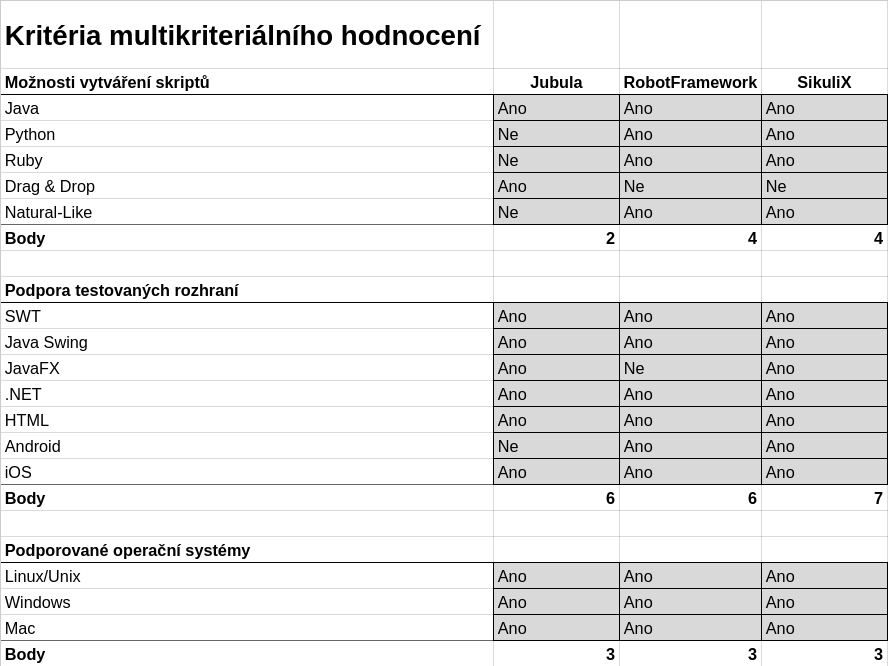
\includegraphics[width=14cm]{img/Kriteria/Kriteria1.png}
		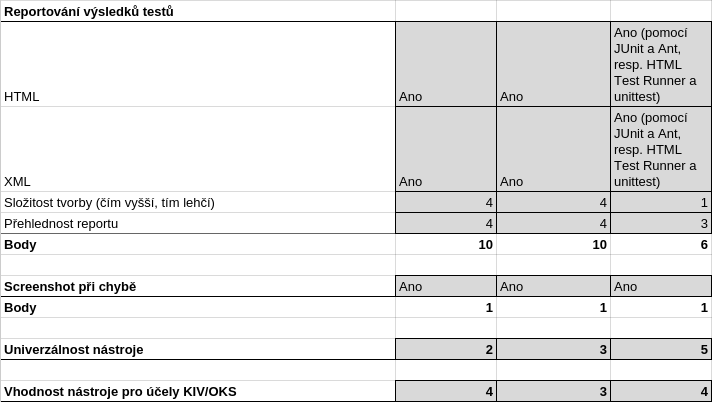
\includegraphics[width=14cm]{img/Kriteria/Kriteria2.png}
	\end{subfigure}
\end{figure}
\begin{figure}[ht]
	\ContinuedFloat
	\begin{subfigure}{\textwidth}
		\centering
		\caption{Výsledek multikriteriálního hodnocení}
		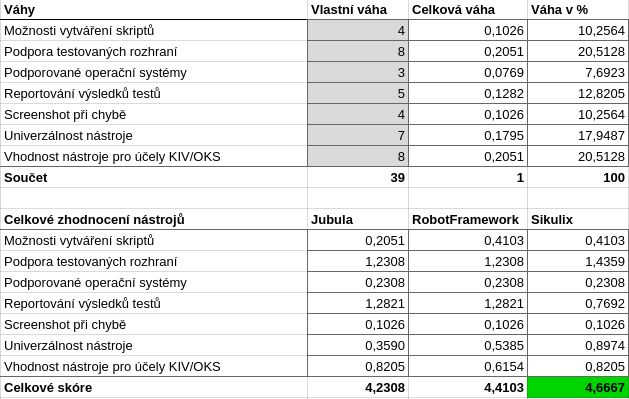
\includegraphics[width=14cm]{img/Kriteria/Kriteria3.png}
	\end{subfigure}
\end{figure}

\chapter{SikuliX}
	\section{Instalace}
	Po stažení balíčku započne instalace jeho spuštěním\footnote{Je potřeba instalace JRE nebo JDK 6 a~vyšší, v~linuxové distribuci balíky \emph{libopencv-core2.4, libopencv-imgproc2.4, libopencv-highgui2.4, libtesseract3} a~\emph{wmctrl} \cite{SikuliX}}. V~průběhu máme na výběr různé možnosti, jak chceme nástroj používat, viz obrázek \ref{Instal}. Např. zda chceme používat SikuliX-IDE a~Python nebo Ruby, jestli budeme používat jiné IDE a~Javu a~zda chceme používat OCR funkce. Zaškrtneme všechna políčka kromě \emph{Ruby (JRuby)} a~klikneme na \emph{Setup Now}. Jsme dotázáni, zda chceme balíčky stáhnout, nebo ukončit instalaci. Zvolíme \emph{Yes}. Další dotaz je na verzi Jythonu, kterou chceme použít, s~upozorněním, že může nastat problém se znaky v~kódování UTF-8. Opět zvolíme \emph{Yes}. Začne vytváření souborů a~měla by se otevřít dvě okna jako na obrázu \ref{InstalOK}, obě potvrdíme tlačítkem \emph{OK}. Pokud vše proběhne v~pořádku, vzniknou v~adresáři soubory podobné těmto\footnote{Může se lišit na různých OS} \emph{runsikulix, SetupStuff, SikuliX-1.1.0-SetupLog.txt, sikulixapi.jar, sikulix.jar}.
	\begin{figure}[ht]
		\centering
		\caption{Instalace SikuliX}
		\label{Instal}
		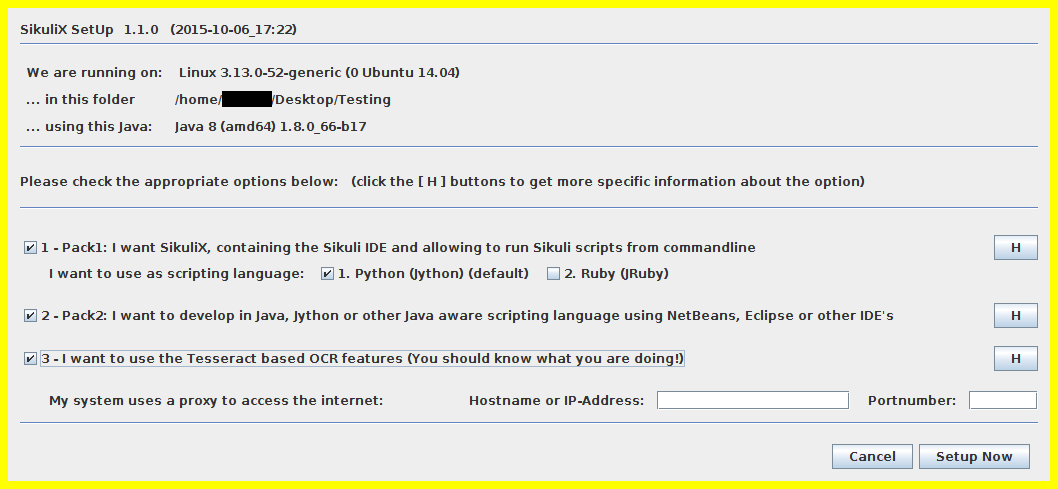
\includegraphics[width=14cm]{img/Instalace/Instalace.png}
	\end{figure}
	\begin{figure}[ht]
		\centering
		\caption{Test instalace}
		\label{InstalOK}
		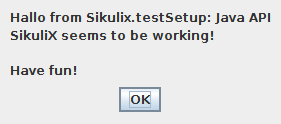
\includegraphics[width=9cm]{img/Instalace/InstalaceOK.png}\\[0.3cm]
		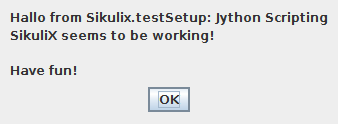
\includegraphics[width=9cm]{img/Instalace/InstalaceOK1.png}
	\end{figure}
	
	\section{SikuliX-IDE}
	Spustit SikuliX-IDE je možné různými způsoby \cite{SikuliX}.
	\begin{enumerate}[leftmargin=*, topsep=-3.5mm, itemsep=-1.5mm]
		\item Spuštěním souboru SikuliX.app (Mac) nebo SikuliX.exe (Windows),
		\item dvojklikem na soubor runsikulix (Linux) nebo runsikulix.cmd (Windows),
		\item z~příkazové řádky příkazem \texttt{java -jar cesta/k/sikulix.jar [volitelne parametry]}.
	\end{enumerate}
	Po spuštění vypadá IDE jako na obrázku \ref{SikuliXIDE}. Jako parametry se v~metodách, ve kterých je to možné, ukazují obrázky vzorů, podle který se na obrazovce nástroj orientuje.
	\begin{figure}[ht]
		\caption{SikuliX-IDE}
		\label{SikuliXIDE}
		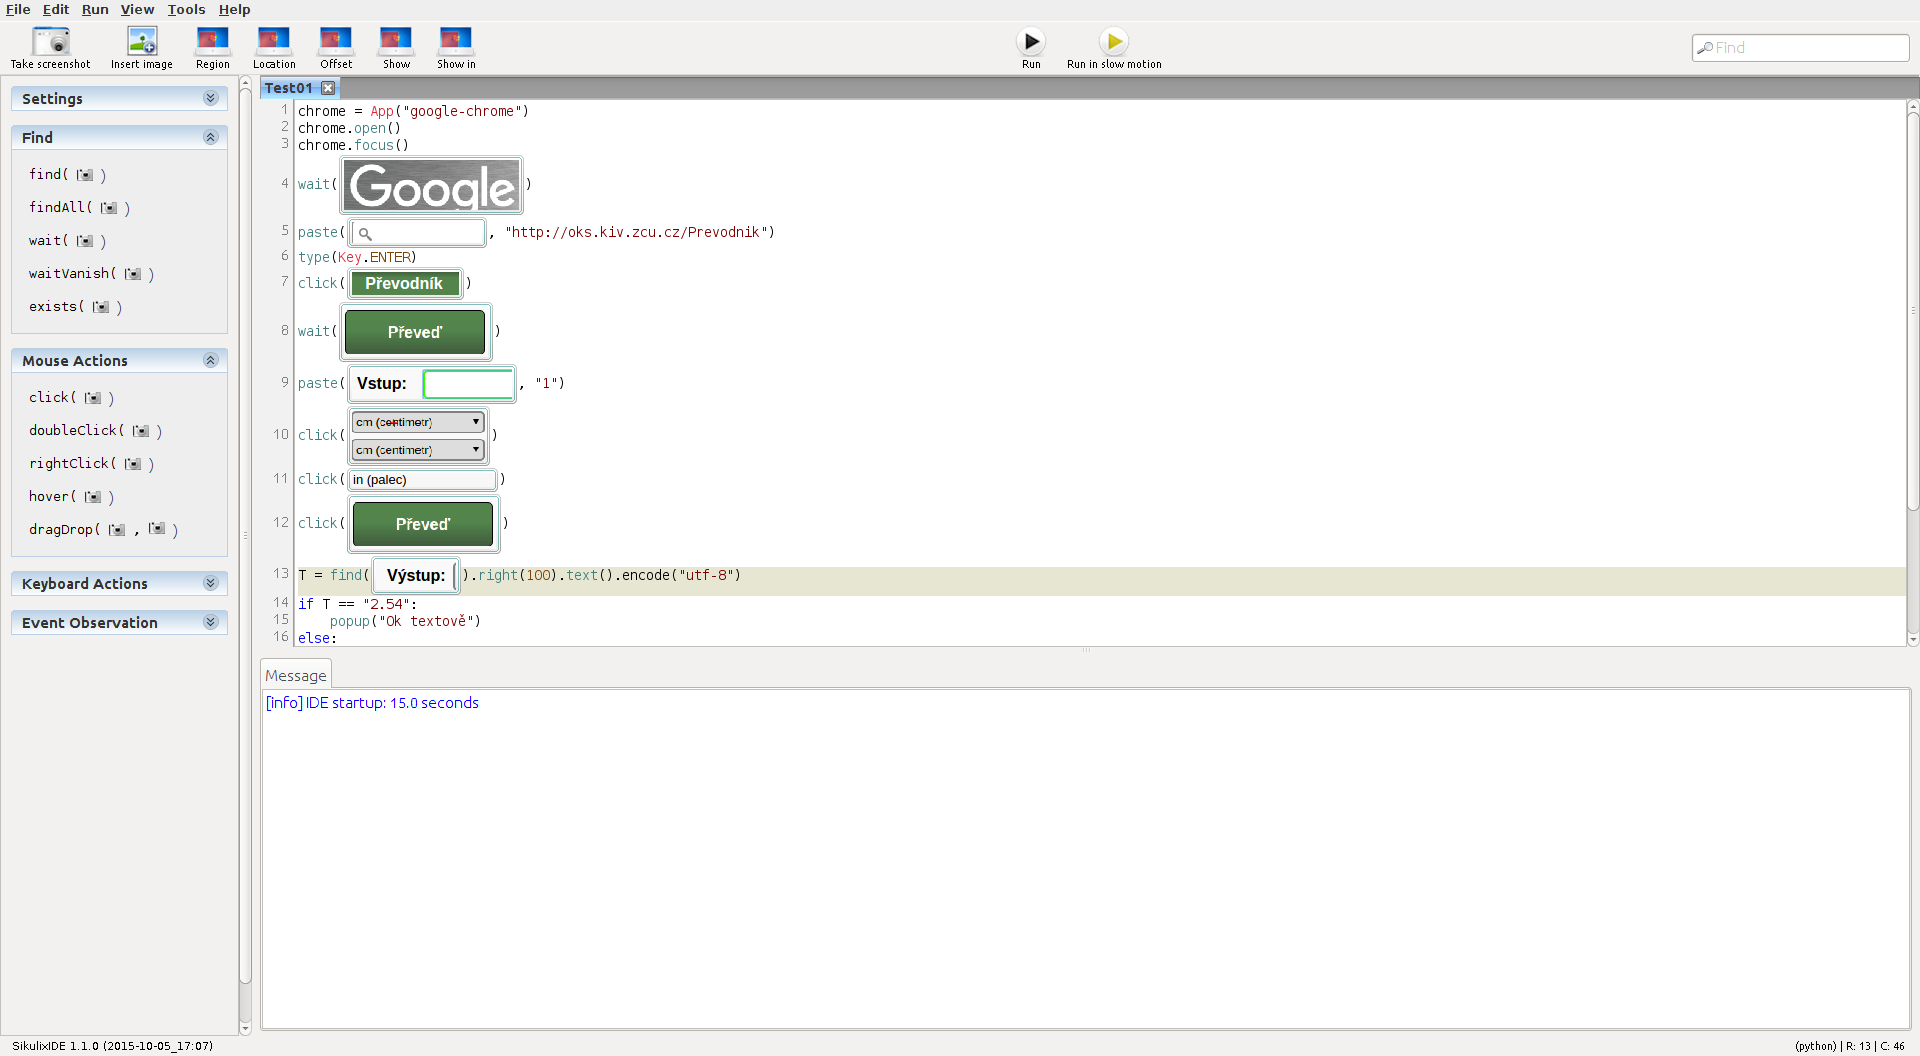
\includegraphics[width=14cm]{img/IDE/SikuliXIDE.png}
	\end{figure}
	
		\subsection{První skript}
		První skript, který jsem v~SikuliX-IDE napsal, demonstruje základní možnost použití nástroje, viz kód \ref{PrvniSkript}. Otevře se prohlížeč, který přejde na adresu \url{http://oks.kiv.zcu.cz/Prevodnik}. Klikne na odkaz \emph{Převodník}, do vstupního pole vloží \emph{1} a~stiskne \emph{Převeď}. Z~pole s~výsledkem přečte text a~porovná jej s~předpokládanou hodnotou \emph{2,54}. Pokud si odpovídají, objeví se vyskakovací okno s~potvrzením, jestliže ne, zobrazí se chybová hláška. Obdobně je tomu následovně, kdy se pouze kontroluje existence obrázku.
		\begin{lstpython}{caption={První skript}, label={PrvniSkript}}
chrome = App("google-chrome")
chrome.open()	#otevre aplikaci definovanou vyse
chrome.focus()	#vybere do popredi jeji okno
#ceka, dokud na obrazovce nenajde obrazek
wait("obr1.png")
#najde na obrazovce obrazek a~vlozi do neho text
paste("obr2.png", "http://oks.kiv.zcu.cz/Prevodnik")
type(Key.ENTER)#simuluje stisk klavesy ENTER
#najde na obrazovce obrazek a~klikne na nej
click("obr3.png")
wait("obr4.png")
paste("obr5.png", "1")
#klikne o~27px vyse a~18px vlevo od nalezeneho obrazku
click(Pattern("obr6.png").targetOffset(-27,-18))
click("obr7.png")
click("obr8.png")
#precte text z~casti, ktera je 100px vpravo od
#nalezeneho obrazku
T = find("obr9.png").right(100).text()
if T == "2.54":
	#pokud rozpoznany text souhlasi se zadanym,
	#otevre se vyskakovaci okno
    popup("Ok textove")
else:
    popError("Chyba")    #jinak se zobrazi chybove okno

if exists("obr10.png"):
	#pokud na obrazovce existuje obrazek, otevre se
	#vyskakovaci okno
    popup("Ok obrazove")
else:
    popError("Chyba")
chrome.close()    #ukonci aplikaci
		\end{lstpython}
		
	\section{Java API}
	Dále jsem se zaměřil na Java API, které SikuliX poskytuje. Pro použití Java API od SikuliX je potřeba mít při překladu a~spuštění nastavený v~classpath \emph{sikulixapi.jar}. Toho docílíme např. tak, že použijeme v~příkazové řádce \texttt{javac -cp sikulixapi.jar:. Test01.java} a~\texttt{java -cp sikulixapi.jar:. Test01}. Syntaxe, kterou SikuliX v~Java API využívá, je velmi podobná té v~Sikuli-IDE, proto ji není třeba vysvětlovat.
	
		\subsection{První testy}
		S~využitím knihoven \emph{JUnit} a~\emph{Log4j} jsem vytvořil čtyři testy, viz kód \ref{PrvniJavaAPI}.
		\begin{lstjava}{caption={První testy Java API}, label={PrvniJavaAPI}}
import org.apache.logging.log4j.LogManager;
import org.apache.logging.log4j.Logger;
import org.junit.AfterClass;
import org.junit.Before;
import org.junit.BeforeClass;
import org.junit.Test;
import org.junit.rules.ErrorCollector;
import org.sikuli.basics.Debug;
import org.sikuli.basics.Settings;
import org.sikuli.script.*;
import javax.swing.*;
import java.time.LocalDateTime;
import static org.junit.Assert.*;

/**
 * @author Jaroslav Klaus
 */
public class Test01 {

  static Logger logger;
  static ErrorCollector collector;
  static Screen s;
  static App chrome;
  static boolean run;

  static {
    System.setProperty("log4j.configurationFile",
      "log-konfigurace.xml");
  }

  private String nazevScreenshotu() {
    LocalDateTime l = LocalDateTime.now();
      return l.getYear() + "" + l.getMonthValue() +
        "" + l.getDayOfMonth() + "" + l.getHour() +
        "" + (l.getMinute() < 10 ? "0" + l.
        getMinute() : l.getMinute()) + "" + l.
        getSecond() + "";
  }

  @BeforeClass
  public static void setUpBeforeClass() {
    logger = LogManager.getLogger();

    Settings.OcrTextSearch = true;
    Settings.OcrTextRead = true;
    Debug.setLogger(logger);
    Debug.setLoggerAll("info");

    collector = new ErrorCollector();
    s~= new Screen();
    chrome = new App("google-chrome");
    chrome.open();
    chrome.focus();
    run = true;
    }

  @AfterClass
  public static void tearDownAfterClass() {
    JOptionPane.showMessageDialog(null, "Script" +
      " dokoncen");
    chrome.close();
  }

  @Before
  public void setUp() {
    try {
      s.wait("png/addressBar.png", 10);
      s.click(new Pattern("png/addressBar.png").
        targetOffset(100, 0));
      s.paste("http://oks.kiv.zcu.cz/Prevodnik");
      s.type(Key.ENTER);
      s.wait("png/zalozkaPrevodnik.png", 5);
    } catch (Exception e) {
      run = false;
      s.capture().save("errors", nazevScreenshotu());
      logger.error(e.getMessage());
    }
  }

  @Test
  public void testPorovnejText() {
    if (run) {
      try {
        s.click("png/zalozkaPrevodnik.png");
        s.wait("png/tlacitkoPreved.png", 5);
        s.paste("png/vstup", "1");
        Match m = s.find("png/jednotky.png");
        m.setTargetOffset(-27, -18);
        m.click();
        s.findText("(metr)").click();
        s.click(new Pattern("png/jednotky.png").
          targetOffset(-27, 18));
        s.find("png/dm.png").click();
        s.click("png/tlacitkoPreved.png");
        String t = s.find("png/vystup.png").right(100).
          text();
        assertEquals(10, Double.parseDouble(t), 0.01);
      } catch (FindFailed | AssertionError e) {
        s.capture().save("errors", nazevScreenshotu());
        logger.error(e.getMessage());
        fail(e.getMessage());
      }
    } else {
      run = true;
      logger.error("setUp neuspesny");
      fail("setUp neuspesny");
    }
  }

  @Test
  public void testPorovnejObraz() {
    if (run) {
      try {
        s.click("png/zalozkaPrevodnik.png");
        s.wait("png/tlacitkoPreved.png", 5);
        s.paste("png/vstup", "1");
        s.click(new Pattern("png/jednotky.png").
          targetOffset(-27, -18));
        s.click("png/inch.png");
        s.click("png/tlacitkoPreved.png");
        assertTrue(s.exists("png/vysledek") != null);
      } catch (FindFailed | AssertionError e) {
        s.capture().save("errors", nazevScreenshotu());
        logger.error(e.getMessage());
        fail(e.getMessage());
      }
    } else {
      run = true;
      logger.error("setUp neuspesny");
      fail("setUp neuspesny");
    }
  }

  @Test
  public void testZkontrolujOdkazObrazekKiv() {
    if (run) {
      try {
        s.click("png/logoKiv.png");
        assertTrue(s.exists("png/zahlaviKiv.png") !=
          null);
      } catch (FindFailed | AssertionError e) {
        s.capture().save("errors", nazevScreenshotu());
        logger.error(e.getMessage());
        fail(e.getMessage());
      }
    } else {
      run = true;
      logger.error("setUp neuspesny");
      fail("setUp neuspesny");
    }
  }

  @Test
  public void testChyba() {
    if (run) {
      try {
        s.wait("png/tlacitkoPreved.png", 5);
        s.paste("png/vstup", "1");
        s.click(new Pattern("png/jednotky.png").
          targetOffset(-27, -18));
        s.findText("(metr)").click();
        s.click("png/tlacitkoPreved.png");
        String t = s.find("png/vystup.png").right(100).
          text();
        assertEquals(100, Double.parseDouble(t), 0.01);
      } catch (FindFailed | AssertionError e) {
        s.capture().save("errors", nazevScreenshotu());
        logger.error(e.getMessage());
        fail(e.getMessage());
      }
    } else {
      run = true;
      logger.error("setUp neuspesny");
      fail("setUp neuspesny");
    }
  }
}
		\end{lstjava}
		
\chapter{Závěr}
Seznámil jsem se s~některými metodami testování grafického uživatelského rozhraní a~zjistil jsem některé důvody používání těchto metod. Dále jsem prozkoumal, které nástroje je k~testování možné využít.

Vybral jsem tři programy, které jsem stručně popsal. Navrhl jsem multikriteriální hodnocení a~provedl jejich podrobné porovnání. Výsledkem byl jeden program, který použiji jako hlavní nástroj v~této práci.

S~aplikací SikuliX, kterou jsem zvolil předchozí činností, jsem se zběžně seznámil a~vytvořil jeden test v~prostředí SikuliX-IDE za použití vlastního jazyka SikuliX. Další čtyři testy jsem zhotovil pomocí Java API, které SikuliX nabízí a~které budu využívat z~důvodu vazby na předmět KIV/OKS.

Jako další se hodlám zaměřit na podrobnější zkoumání používání nástroje. Také připravím sadu ukázkových testů a~funkční scénáře.
		
\appendix
\bibliographystyle{csplainnat}
\bibliography{bakalarka}
\end{document}
